\documentclass[border=2pt]{standalone}
\usepackage{tikz}
\begin{document}
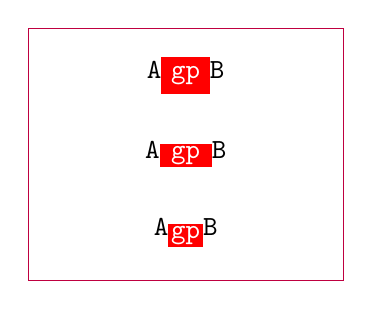
\begin{tikzpicture}
  \draw[red!75!blue] (-2,.6) rectangle (2,-2.6);
  \node at (0,0) {\tt A\tikz[baseline]{\node[rectangle,fill=red,anchor=base]{\textcolor{white}{gp}};}B};
  \node at (0,-1) {\tt A\tikz[baseline]{\node[rectangle,fill=red,inner xsep=.4em,inner ysep=.2ex,anchor=base]{\textcolor{white}{gp}};}B};
  \node at (0,-2) {\tt A\tikz[baseline]{\node[rectangle,fill=red,inner sep=1pt]{\textcolor{white}{gp}};}B};
\end{tikzpicture}
\end{document}
